\chapter{FPGAs}
{
\large
Every section is arranged like follows:
\begin{itemize}
\item Abstract\\
	The abstract part of paper.
\item Content\\
	The main idea of paper.
\item Results\\
	The experiment implementation.
\item Conclusion \\
	The conclusion part of paper.
\end{itemize}
}
\section{Performance Comparison of FPGA, GPU and CPU in Image Processing 2009}
%\noindent {\Large \textbf{Abstract}}\\
\subsection{Abstract}
\indent \textbf{Many applications in image processing have high inherent
parallelism}. FPGAs have shown very high performance in
spite of their low operational frequency by fully extracting
the parallelism. In recent micro processors, it also becomes
possible to utilize the parallelism using multi-cores which
support improved SIMD instructions, though programmers
have to use them explicitly to achieve high performance. Re-
cent GPUs support a large number of cores, and have a po-
tential for high performance in many applications. \textbf{However,
the cores are grouped, and data transfer between the groups
is very limited.} Programming tools for FPGA, SIMD in-
structions on CPU and a large number of cores on GPU have
been developed, but it is still difficult to achieve high perfor-
mance on these platforms. In this paper, we compare the per-
formance of FPGA, GPU and CPU using three applications
in image processing; two-dimensional filters, stereo-vision
and k-means clustering, and make it clear which platform is
faster under which conditions.

\begin{figure*}[t]
\centering
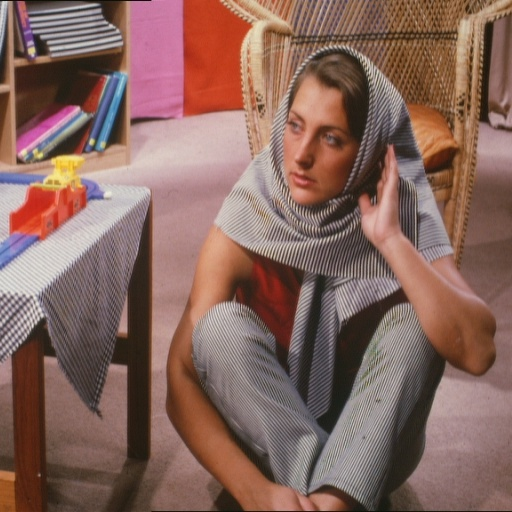
\includegraphics[width=0.9\textwidth]{Barbara.jpg}
\caption{传统提升小波计算过程}
\label{figWavelet}
\end{figure*}


\subsection{Content}
Compared three applications: two-dimension filters, stereo-vision, k-means clustering.\\

The high performance of FPGA comes from its flexibility which makes it possible to realize the fully optimized circuit for each application, and a large number of on-chip memory banks which supports the high parallelism.{\bfseries FPGA can achieve extremely high
performance in many applications in spite of its low op-
erational frequency}.\\

GPU cores are grouped, the data transfer between groups is very slow. \\

\noindent\textbf{GPU Analysis}\\
\indent It consists of 10 thread processor clus-
ters. A thread processor cluster has three streaming mul-
tiprocessors, eight texture filtering units, and one level-1
cache memory. Each streaming multiprocessor has one in-
struction unit, eight stream processors (SPs) and one local
memory (16KB). Thus, GTX280 has 240 SPs in total. Eight
SPs in a streaming multiprocessor are connected to one in-
struction unit. This means that the eight SPs execute the
same instruction stream on different data.

\noindent \textbf{Two-Dimensional Filters}\\
\indent The computational complexity of filters is $O(w \times w)$, and $w$ is radius of filter.
\begin{figure}[!hbtp]
\centering
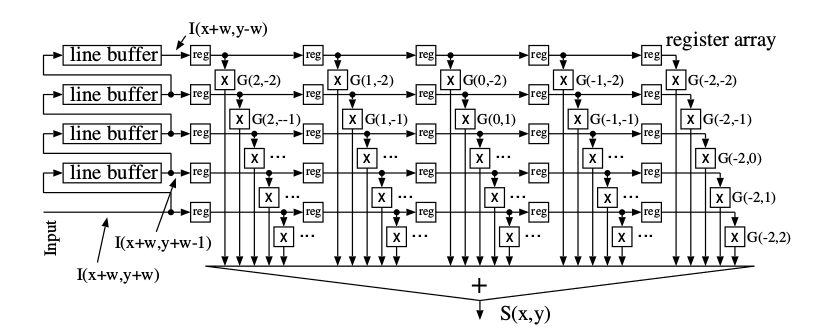
\includegraphics[width=0.9\textwidth]{FPGAs/Paper1_1_Cirsuitsfornon-separablefilters}
\caption{Circuits for non-separable filters}
\label{fig1.1}
\end{figure}\\
Fig\ref{fig1.1} shows the filter is $5 \times 5$ case.\\
\noindent \textbf{Stereo Vision}\\
\indent This application is to get the distance to the location obtained from the two camera's disparity.The sum of absolute difference (SAD) is widely used to compared the windows because of its simplicity\index{SAD}. 
More details can be found in paper\cite{asano2009performance}.
\noindent\textbf{K-means Clustering}\\
\indent More details can be found in paper \cite{asano2009performance}.
\subsection{Results}
\begin{itemize}
\item Xilinx XC4VLX160.
\item GeForce 280GTX, 1 GB DDR3, CUDA version 2.1.
\item Intel Core2 Extreme QX6859.
\end{itemize}
The time to download images from main memory is not included. CPU has four cores, FPGA is fixed to 100MHz. Fig is the performance of two-dimension filters.
\begin{figure}[!hbtp]
\centering
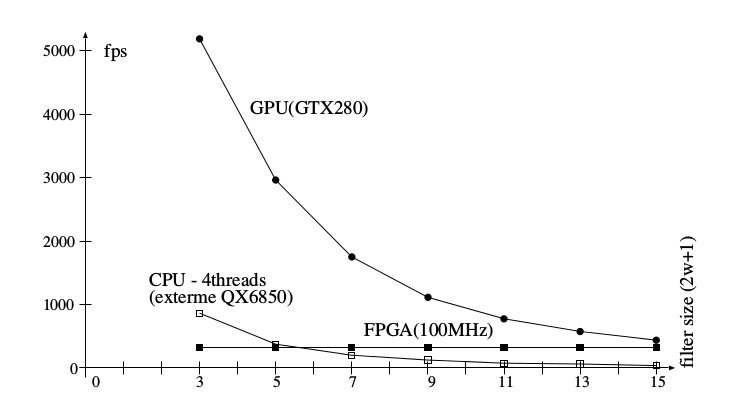
\includegraphics[width=0.9\textwidth]{FPGAs/Paper1_1_PerformanceofTwo-DimensionFilters}
\caption{Performance of two-dimensional filters}
\label{fig1.2}
\end{figure}\\
\indent GPU is the fastest for all tested filter size.In this
problem, filters can be applied to each pixel in the image in-
dependently without using shared variables. So, GPU can
show its best performance.\\

{\color{purple} In the later two applications, the performance FPGA is much better than GPU.}
\subsection{Conclusion}
\indent We have compared the performance of GPU with FPGA
and CPU (quad-cores) using three simple problems in im-
age processing. GPU has a potential for achieving almost
the same performance with FPGA. The number of cores in
GTX280 is 240.Considering the trade-offs between the operational frequency of GPU (more than 10 times faster), and
the fine-grained parallelism in FPGA, this seems to be a
natural consequence. However, GPU can show its potential
only for naive computation methods, in which all pixels can
be processed independently. For more sophisticated algorithms  
which use shared arrays, GPU can not execute those
algorithms because of its very small local memory, or can
not show good performance because of the memory access
limitation caused by its memory architecture. GPU is slower
than CPU in those algorithms (it may be possible to realize
much better performance if we can find algorithms which
can get around the limitations, but we could not find them).
The performance of CPU is 1/12 - 1/7 of FPGA, which
means that CPU with quad-cores can executes about 1/10
operations of FPGA in a unit time (the same algorithms are
executed on CPU and FPGA). The performance of FPGA
is limited by the size of FPGA and the memory bandwidth.
With a latest FPGA board with DDR-II DRAM and a larger
FPGA, it possible to double the performance by processing
twice the number of pixels in parallel.\\
\indent We have the following issues which have to be consid-
ered. We have compared the performance using only three
problems. The performances of the programs on GPU and
CPU are not fully tuned up. In the comparison, power con-
sumption and costs are not considered.

\section{Fast FPGA Prototyping for real-time image processing with very high-level synthesis 2017}
\subsection{Abstract}
Programming in high abstraction level can facilitate the development of digital signal processing systems. In the recent 20 yeahs, HLS has made significantly progress. However, due to the high complexity and computational intensity, image processing algorithms usually necessitate a higher abstraction environment than C-synthesis, and the current HLS tools do not have the ability of this kind. This paper presents a conception of very high-level synthesis method which allows fast prototyping and verifying the FPGA-based image processing designs in the MATLAB environment. We build a heterogeneous development flow by using currently available tool kits for verifying the proposed approach and evaluated it within two real-life applications. Experiment results demonstrate that it can effectively reduce the complexity of the development by automatically synthesizing the algorithm behavior from the user level into the low register transfer level and give play to the advantages of FPGA related to the other devices.
\subsection{Content}
Advanced Digital Sciences Center(ADSC) of the University of Illinois reported that FPGA can achieve a speedup to 2-2.5x and save 84-92\% of the energy consumption comparing to Graphics Processing Units(GPUs). ADSC indicates also that a manual FPGA design may consume 6-18 months and even years for a full custom hardware, while the GPUs(CUDA) based designed only 1-2 weeks. \\

Fig\ref{fig1.3} show the Gasjki-Kuhn's Y-chart comparing the conventional RTL with the HLS-based design flows.\\
\begin{figure}[!hbtp]
\centering
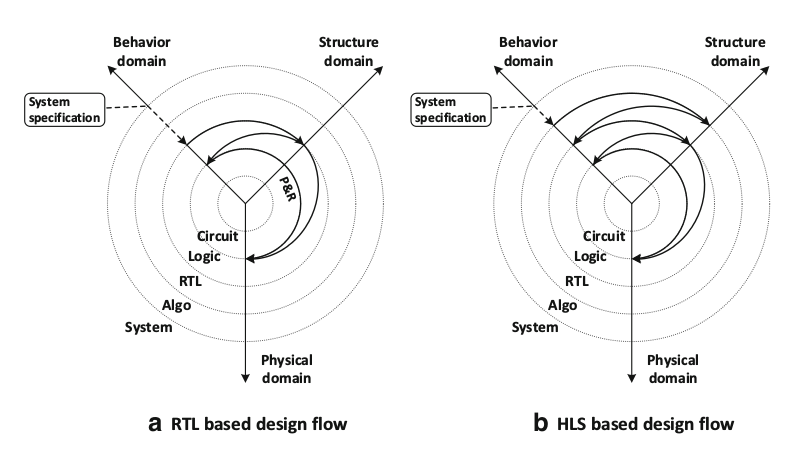
\includegraphics[width=0.9\textwidth]{FPGAs/Paper1_2_Comparison}
\caption{Comparison of RTL- and HLS-based design flows by using Gasjki-Kuhn's Y-chart: full lines indicate the automated cycles, while dotted lines the manual cycles.}
\label{fig1.3}
\end{figure}
The challenges of MATLAB-to-RTL synthesis include:
\begin{itemize}
\item Operators in MATLAB perform different operations depending on the type of the operands, whereas the functions of the operators in RTL are fixed.
\item MATLAB includes very simple and powerful vector operations such as the concatenation ``[ ]'' and column operators ``$x(:)$'' or ``end'' construct, which can be quite hard to map to RTL.
\item MATLAB supports ``polymorphism'' whereas RTL does not. More precisely, functions in MATLAB are genetic and can process different types of input parameters. In the behaviors of RTL, each parameter has only a single given type, which cannot change.
\item MATLAB supports dynamic loop bounds or vector size, whereas RTL requires users to initialize explicitly them and cannot do any changes during the synthesis.
\item The variables in MATLAB can be reused for different contents (different types), whereas RTL does not, as each variable has one unique type.
\end{itemize}
\par\indent Two complex image processing applications: Kubelka-Munk genetic algorithm(KMGA) for the multispectral image based skin lesion assessments \& level set method(LSM)-based algorithm for very high-resolution(VHR) satellite image segmentation.\index{KMGA}\index{LSM}\index{VHR}.